\documentclass[10pt]{article}

\usepackage{geometry}
\geometry{margin = 2em, left=2.5cm, top =6em, headheight=\paperheight}
\usepackage[export]{adjustbox}
\usepackage{array}
\usepackage{amsmath}
\usepackage{amsfonts}
\usepackage{fancyhdr}
\pagestyle{fancy}
\fancyhf{}
\lhead{Algebra II}
\chead{Function  Characteristics - Increasing and Decreasing}
\rhead{Action Opportunity B, Page \thepage}
\usepackage{lastpage}
\usepackage{xcolor}
\usepackage{enumitem}
\usepackage{pifont}
\usepackage{graphicx}
\graphicspath{{../img}}
\usepackage{pgfplots}
\pgfplotsset{compat=1.18}
\usepackage{tabularx}

\newcommand{\R}{\mathbb R}
\newcommand{\e}{{\rm e}}
\newcommand{\pobr}[1]{\left\langle#1\right\rangle}
\newcommand{\norm}[1]{\lVert #1 \rVert}
\newcommand{\abs}[1]{\lvert #1 \rvert}

\DeclareMathOperator{\xd}{d\!}
\DeclareMathOperator{\proj}{proj}

\title{}
\date{}

\begin{document}
\noindent
{\large
First Name \rule{6em}{.1pt}\hspace{\stretch{1}}Last Name \rule{6em}{.1pt}\hspace{\stretch{1}} Date \rule{1.5em}{.1pt} -- \rule{1.5em}{.1pt} -- \rule{1.5em}{.1pt}\hspace{\stretch{1}} Period \rule{2em}{.1pt}\hspace{\stretch{1}} Score \rule{2em}{.1pt}
}
\vspace{1em}

\begingroup
\renewcommand{\arraystretch}{1.5}
\begin{center}
\tiny
{
\begin{tabularx}{\textwidth}{|X|X|X|X|X|X|}
\hline
\bf BE PRECISE & \centerline{Integrating} & \centerline{Applying} & \centerline{Practicing} & \centerline{Acquiring} & \centerline{Awaiting Evidence} \\
\hline
I can calculate accurately and efficiently, and be precise in all of my math.&
Selects and applies the correct procedure and solves all routine AND integrating problems.

AND

Expresses the answer to the correct level of precision needed for the problem (including the correct rounding, units, math symbols, labeling, graphing, vocab…)
&Selects and applies the correct procedure and solves all routine problems.


AND

Expresses the answer to the correct level of precision needed for the problem (including the correct rounding, units, math symbols, labeling, graphing, vocab…)
&Selects and applies the correct procedure and solves most routine problems.


AND

Expresses the answer to the correct level of precision needed for the problem (including the correct rounding, units, math symbols, labeling, graphing, vocab…)
&Selects and applies the correct procedure and solves some routine problems.


AND

Attempts to express the answer to the correct level of precision needed for the problem (including the correct rounding, units, math symbols, labeling, graphing, vocab…).
&Selects and attempts to apply the correct procedure for some routine problems.\\
\hline
\bf Criteria&\multicolumn{5}{l|}{\parbox[c][4em]{.8\textwidth}{}}\\
\hline
\end{tabularx}
}
\end{center}
\endgroup
\vspace{1em}
\begin{enumerate}

\item Consider the interval $[-3,2]$.
\begin{enumerate}
\item Shade the segment represented by the interval above on the number line. Use $\bullet$ to indicate a closed endpoint, and $\circ$ to indicate an open endpoint.
\vspace{1em}
\begin{center}
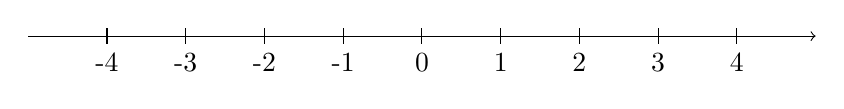
\begin{tikzpicture}
  \draw[->] (-5,0) -- (5,0);
  \foreach \x in {-4,..., 4}
    \draw (\x,0.1) -- (\x,-0.1) node[below] {\x};
\end{tikzpicture}
\end{center}
\vspace{2em}
\item Write the interval as an inequality. \rule{12em}{0.1pt}

\end{enumerate}
\item The following chart summarizes the New York house price index in 2021 through 2025.
\begin{figure}[h]
\centering
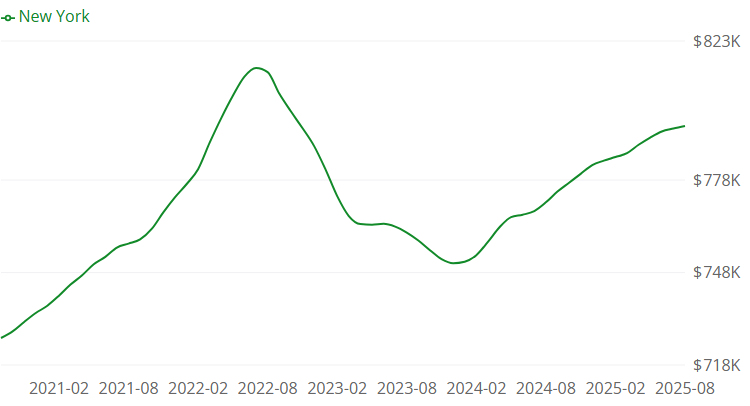
\includegraphics[width=.6\textwidth]{new-york-house-price-2021-2025.png}
\end{figure}

\begin{enumerate}
\item
On the horizontal axis, box the whole period(s) between 2022-08 and 2025-08 when the housing prices were increasing. 
\item
On the vertical axis, box net gain over the increasing period(s) you identified above. 
\end{enumerate}
\clearpage
\item {\bf Direction.} On the graphs below, use $\bigwedge$ to label the turning point from inceasing to decreasing,  $\bigvee$ to label the turning point from decreasing to increasing. On the $x$-axis, box the increasing interval, and shade the decreasing interval.
\begin{enumerate}
\item\ 
\begin{center}
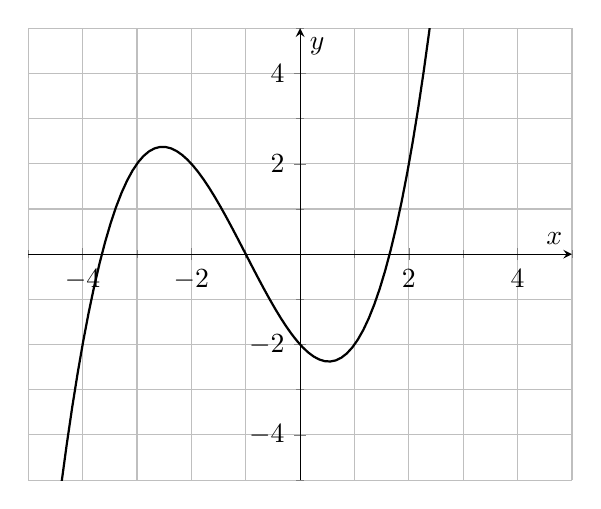
\begin{tikzpicture}
\begin{axis}[
    xlabel={$x$},
    ylabel={$y$},
    grid=both,
    minor tick num=1,
    axis lines=middle,
    xmin=-5,xmax=5,
    ymin=-5,ymax=5,
    domain=-5:5,
    samples=100,
    width=0.7\textwidth
]
\addplot[thick]{(x+3)*(x+2)*(x-2)/3+2};
\end{axis}
\end{tikzpicture}
\end{center}
\vspace{\stretch{1}}
\item\ 
\begin{center}
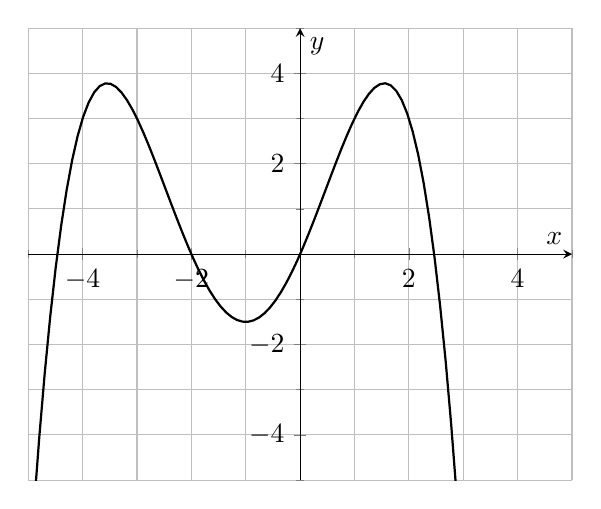
\begin{tikzpicture}
\begin{axis}[
    xlabel={$x$},
    ylabel={$y$},
    grid=both,
    minor tick num=1,
    axis lines=middle,
    xmin=-5,xmax=5,
    ymin=-5,ymax=5,
    domain=-5:5,
    samples=100,
    width=0.7\textwidth
]
\addplot[thick]{-(x+1+3)*(x+1+2)*(x+1-2)*(x+1-3)/8 + 3};
\end{axis}
\end{tikzpicture}
\end{center}
\end{enumerate}

\end{enumerate}
\end{document}